\section{MetaMask}
	\subsection{What is MetaMask}
	MetaMask\glosp is a browser extension that manages your Ethereum\glosp digital wallet\glosp and 
	allows you to send and receive Ethers\glosp (CCs\glosp in \textit{Soldino}). 
	\\
	Note that MetaMask\glosp has to be installed in your browser as long as you want 
	to use the platform: removing it from your browser will render you unable 
	to use \textit{Soldino}.
	\subsection{Installation}
	After entering \textit{Soldino}'s homepage you should check if you have MetaMask\glosp 
	installed. If not, you can check this by looking for its icon on the top right of your browser.
	\begin{figure}[H]
		
\includegraphics[width=7cm]{res/images/metamask_icon.png}
		\centering
		\caption{MetaMask's icon}
	\end{figure}
	\noindent If you have it proceed with the configuration of your account.
	Otherwise, watch the video introduction, click the link under the video and 
	follow the instructions to download it. 
	\begin{figure}[H]
		
\includegraphics[width=7cm]{res/images/metamask_download.png}
		\centering
		\caption{Introduction to MetaMask}
	\end{figure}
	\noindent After the installation process is 
	complete you will see MetaMask\glo's icon on the top right of your browser. A 
	new window will then open where you will have to configure your account.\\
	The download page can also be found at \url{https://metamask.io/}.
	\subsection{Configuration}
	Click on MetaMask's icon on the top right of your browser, and set up your 
	Ethereum\glosp digital wallet\glosp by following the instructions. You can either 
	create a new account or import an existing one using the 12 words seed phrase
	that was previously given to you.
	\begin{figure}[H]
		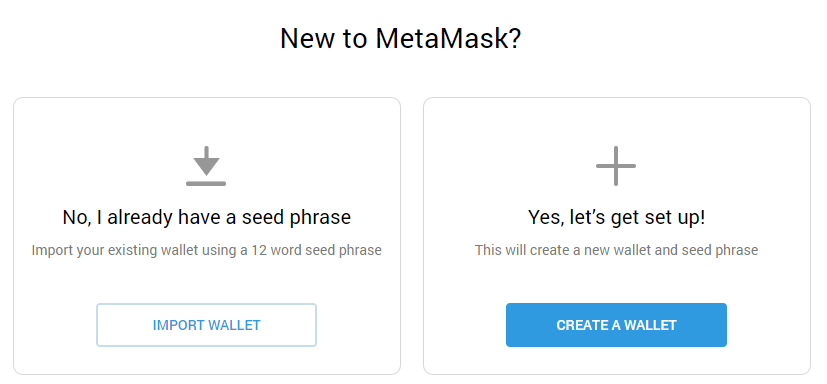
\includegraphics[width=15cm]{res/images/metamask_select.png}
		\centering
		\caption{MetaMask setup}
	\end{figure}
	\noindent After setting up your account you will be able to join and use 
	\textit{Soldino}.
	\subsection{Operations}
	Every time you make a operation that changes the state of the Ethereum\glosp 
	network MetaMask\glosp will open a pop-up window that shows you its total cost.
	From this window you will be able to accept or decline the transaction.\\
	\begin{figure}[H]
		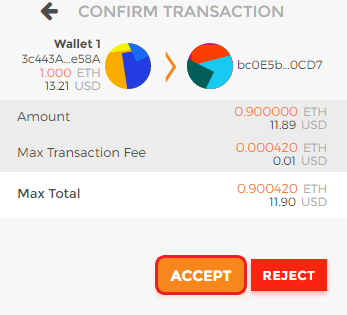
\includegraphics[width=9cm]{res/images/metamask_transaction.png}
		\centering
		\caption{Example of a MetaMask transaction}
	\end{figure}
	\noindent 
	Every change made on the Ethereum\glosp Network has a cost and it is called 
	Gas\glosp and is measured in GWEI, a billionth of an Ether\glo. When you 
	make a transaction you can choose whether it should have a high or low 
	priority: higher priority will consume more Gas than a lower one but will 
	be mined quicker. We do not recommend changing the priority for 
	operations made in \textit{Soldino}.
		\subsubsection{Operations costs}
		In the table that follows you can find an estimate of the costs of operations 
		you can make in \textit{Soldino}.
		\begin{table}[H]
			\centering\renewcommand{\arraystretch}{1.5}
			\caption{Costs of operations}
			\vspace{0.2cm}
			\begin{tabular}{c c c}
				
				\rowcolorhead
				{\colorhead \textbf{Operation}} &
				{\colorhead \textbf{Average gas cost}} & 
				{\colorhead \textbf{Average Cubit cost}} \\
				
				\rowcolorlight
				{\colorbody Creating a citizen account} & {\colorbody 102098} & 
				{\colorbody 0.34}  
				\\
				
				\rowcolordark
				{\colorbody Creating a business account} & {\colorbody 104598} & 
				{\colorbody 0.35}  
				\\	
				
				\rowcolorlight
				{\colorbody Adding a new product} & {\colorbody 182044} & 
				{\colorbody 0.60} 
				\\
				
				\rowcolordark
				{\colorbody Modifying a product} & {\colorbody 97986} & 
				{\colorbody 0.33} 
				\\
				
				\rowcolorlight
				{\colorbody Deleting a product} & {\colorbody 42338} & 
				{\colorbody 0.14} 
				\\
				
%				\rowcolordark
%				{\colorbody AZIONE} & {\colorbody PREZZO IN GAS} & 
%				{\colorbody PREZZO IN CC} 
%				\\
%				
%				\rowcolorlight
%				{\colorbody AZIONE} & {\colorbody PREZZO IN GAS} & 
%				{\colorbody PREZZO IN CC} 
%				\\
%				
%				\rowcolordark
%				{\colorbody AZIONE} & {\colorbody PREZZO IN GAS} & 
%				{\colorbody PREZZO IN CC} 
%				\\
%				
%				\rowcolorlight
%				{\colorbody AZIONE} & {\colorbody PREZZO IN GAS} & 
%				{\colorbody PREZZO IN CC} 
%				\\
			\end{tabular}
		\end{table}
	\noindent The costs shown above were calculated 2019-03-25.